\chapter{Relational Database Service (RDS)}\label{ch:relational-database-service}
% Evie was here…
Amazon RDS service allows a user to create a fully-featured and highly-available SQL database that is automatically
replicated to another availability zone. (TODO: Oops, no multi-az) This means that if the primary database becomes
unavailable, there is automatic failover providing redundancy for all the data stored within.

To create an Amazon RDS instance, a suitable name/identifier for the database is required before created as well as a
selection for the resource limits for the virtual server.
The database requires a username and passphrase, although for additional security there is the option to automatically
generate a passphrase.

Afterwards, the type of SQL database required (such as MySQL, PostgreSQL, MariaDB or others) will be selected and then
the database should begin provisioning.

\begin{figure}[!htbp]
    \centering
    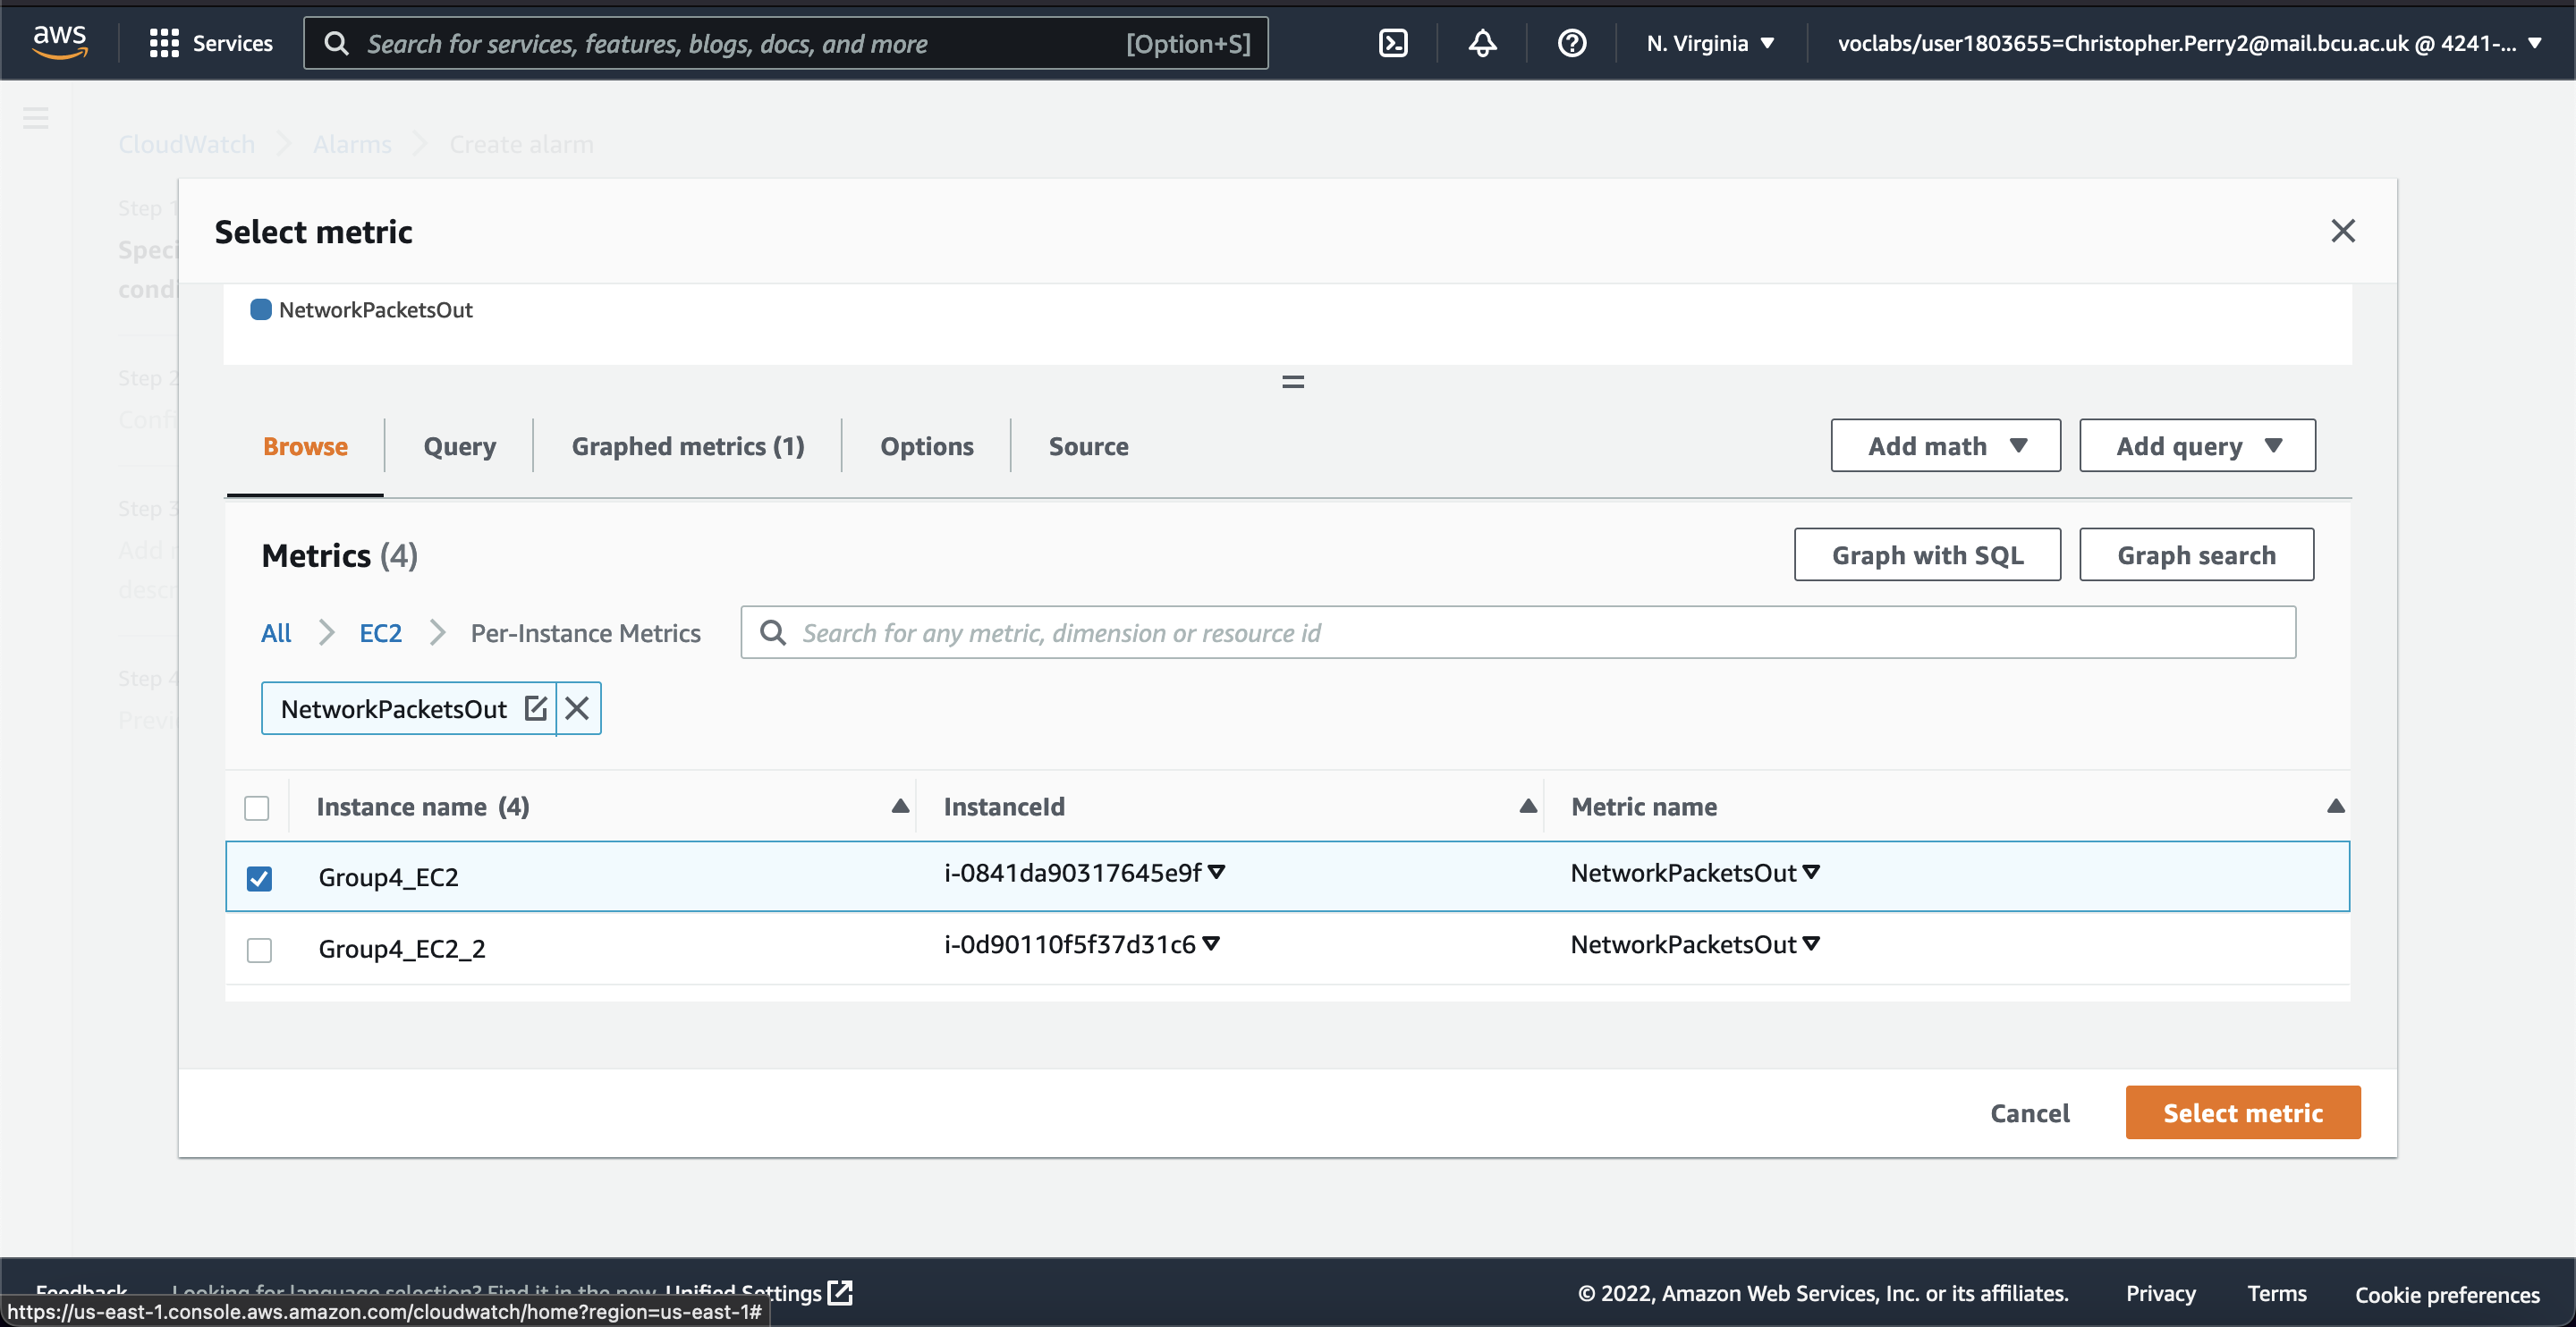
\includegraphics[width=\textwidth]{resources/cloudwatch/cloudwatch-metric-selection}
    \caption{Selection of CloudWatch metric for EC2 instance.}
    \label{fig:cloudwatch-metrics}
\end{figure}